\chapter{Quantum Estimation, the Rayleigh Limit, and SPADE Sub-Rayleigh Resolution}
\label{chap:e12}

\begin{chapteropening}
For more than a century, when astronomers judged whether "two stars can be separated," they relied on the same sentence: the main peaks of the two diffraction spots must be far enough apart that a dip can be seen between them. This is the Rayleigh criterion. But stop and think: if I already \emph{know} that there are two equally bright stars up there, and I simply do not know how far apart they are, then does "no visible dip" really mean "the separation cannot be measured"? This chapter overhauls the whole notion of "resolution": we no longer ask "can the image plane be split into two peaks," but rather "given this many photons and this particular point spread function, how precisely can I estimate the angular separation of the two stars?" In other words, we upgrade the imaging criterion into an \textbf{estimation problem}. Once the question is posed this way, a startling fact emerges: when the two stars sit very close together, ordinary imaging throws away the separation information at a rate $\propto s^2$ (this is the so-called Rayleigh curse), yet that information \emph{never actually leaves the light field}; it is simply missed by the clumsy method of "recording position pixel by pixel." A different measurement (first projecting the light onto a set of spatial modes and then counting photons, that is, SPADE) can recover it. This chapter starts from a Gaussian point spread function and, without skipping a single step, derives all of this; finally it carries the same Fisher-information language over to kilometre-scale long-baseline intensity interferometry, to see where the weak spots of each of the two engineering routes lie.
\end{chapteropening}


\section{From "can it be split into two peaks" to "how precisely can the separation be estimated"}
\label{sec:e12-rayleigh}

Let us first sketch out the most familiar line of reasoning. A telescope of aperture $D$, working at wavelength $\lambda$, imaging a point source, produces not a point but a small diffraction spot (an Airy disk in the case of a circular aperture). For two point sources to "be separated," the classical Rayleigh criterion says: the main peak of one source's diffraction spot must fall exactly on the first dark ring of the other source's diffraction spot. For a circular aperture this angular separation is

\begin{equation}
  \theta_{\rm R}=1.22\,\frac{\lambda}{D}.
  \label{eq:e12-rayleigh}
\end{equation}
\begin{formulaexplain}
$\theta_{\rm R}$: the Rayleigh angular scale (radians). $\lambda$: the observing wavelength (metres). $D$: the telescope aperture (metres). The coefficient $1.22$ comes from the position of the first dark ring of the circular-aperture Airy disk. It is an \emph{imaging} criterion, not the ultimate limit of estimation.
\end{formulaexplain}

Let us go symbol by symbol and plug in a real number. $\theta_{\rm R}$ is in radians; to convert to the milliarcseconds customary in astronomy, multiply by $206265\times10^3$ (because $1\,\mathrm{rad}=206265''=2.06\times10^{8}\,\mathrm{mas}$). A telescope of $D=8\,\mathrm{m}$, at $\lambda=500\,\mathrm{nm}=5\times10^{-7}\,\mathrm{m}$, gives
\[
  \theta_{\rm R}=1.22\times\frac{5\times10^{-7}}{8}
  =7.6\times10^{-8}\,\mathrm{rad}
  \approx15.7\,\mathrm{mas}.
\]
For a $30\,\mathrm{m}$ giant mirror, at the same wavelength this is about $4.2\,\mathrm{mas}$. These numbers tell us how big the diffraction spot is, but they do \emph{not} tell us "whether two stars separated by only 1 milliarcsecond can actually be measured or not." To answer the latter question, we need a different language.

To make the algebra transparent, we replace the two-dimensional circular aperture with a one-dimensional Gaussian point spread function (PSF for short). This is not laziness: the Gaussian PSF preserves the core feature of "a response kernel of finite width," while letting every integral be done by hand. Write

\begin{equation}
  h(x)=\frac{1}{\sqrt{2\pi}\,\sigma}\,
       \exp\!\left(-\frac{x^{2}}{2\sigma^{2}}\right).
  \label{eq:e12-gaussian-psf}
\end{equation}
\begin{formulaexplain}
$h(x)$: the normalized point spread function (its units are the reciprocal of length or angle, and it integrates to 1). $x$: the image-plane coordinate or equivalent angular coordinate. $\sigma$: the PSF width, playing the role of the diffraction-spot radius, of order $0.4\lambda/D$ to $0.5\lambda/D$.
\end{formulaexplain}

Here, if $x$ is an angular coordinate, then $\sigma$ is the angular width $\sigma_\theta$, of order $0.5\lambda/D$: for the 8-metre mirror above, $\lambda/D=6.25\times10^{-8}\,\mathrm{rad}\approx12.9\,\mathrm{mas}$, so $\sigma_\theta\approx0.5\times12.9\approx6\,\mathrm{mas}$. It is a single number for "how fat the diffraction spot is."

Now place two \textbf{equally bright, mutually incoherent} point sources, put their centroid at the origin, one at $+s/2$ and one at $-s/2$, so the angular separation is $s$. "Mutually incoherent" is crucial: it means we must add the \emph{intensities} of the two stars separately, rather than adding the amplitudes and then squaring (this boundary was emphasized repeatedly in Chapter~\ref{chap:e10} when discussing spatial coherence). Hence the probability density for a single detected photon to land at image-plane position $x$ is the equal-weight average of two shifted PSFs:

\begin{equation}
  p(x\mid s)=\tfrac12\,h\!\left(x-\tfrac{s}{2}\right)
            +\tfrac12\,h\!\left(x+\tfrac{s}{2}\right).
  \label{eq:e12-direct-prob}
\end{equation}
\begin{formulaexplain}
$p(x\mid s)$: the probability density, given separation $s$, that one photon lands at $x$. The two $h$ terms come from the stars on either side of the centroid, and the coefficients $\tfrac12$ express equal brightness. What direct imaging sees is precisely this intensity superposition of the two diffraction spots.
\end{formulaexplain}

\paragraph{The key step: at small separations the first effect is "fattening," not "splitting"}
\label{sec:e12-taylor}

Now we carry out the first, and most counterintuitive, derivation of the chapter. We want to see: when $s\ll\sigma$, how exactly does $p(x\mid s)$ vary with $s$? The tool we use is the \textbf{Taylor expansion}, expanding a slightly shifted function in terms of its value and successive derivatives at the original point. For a shift of $\pm s/2$, expanding to second order:

\[
  h\!\left(x\pm\tfrac{s}{2}\right)
  =h(x)\;\pm\;\frac{s}{2}\,h'(x)
   \;+\;\frac{1}{2}\left(\frac{s}{2}\right)^{2}h''(x)
   \;+\;\mathcal{O}(s^{3})
  =h(x)\pm\frac{s}{2}h'(x)+\frac{s^{2}}{8}h''(x)+\mathcal{O}(s^{3}).
\]

Substitute these two into Eq.~\eqref{eq:e12-direct-prob}. Note the weight $\tfrac12$, and that \textbf{the first-order terms have opposite signs}: one star moves right, one moves left, and $\pm h'(x)$ cancel exactly. Thus

\[
  p(x\mid s)
  =\tfrac12\Big[h+\tfrac{s}{2}h'+\tfrac{s^{2}}{8}h''\Big]
  +\tfrac12\Big[h-\tfrac{s}{2}h'+\tfrac{s^{2}}{8}h''\Big]
  +\mathcal{O}(s^{4})
  =h(x)+\frac{s^{2}}{8}\,h''(x)+\mathcal{O}(s^{4}).
\]

Pause and savour this result. \emph{The separation $s$ enters the image plane at lowest order as $s^2$, and it does so through the second derivative $h''$}. The second derivative is negative at the Gaussian peak and positive in the two wings; its effect is to "press the peak down a little and lift the shoulders up a little", in other words, to make the diffraction spot \textbf{fatter}. So the first thing two nearby stars do in the image plane is not "split into two peaks" but "broaden slightly overall." "No visible two peaks" therefore \emph{does not at all mean} "no information"; the information is hidden in a second-order small quantity, and ordinary imaging merely finds it very hard to dig out of the noise.

This leads naturally to the question of the next section: this information hidden in the second-order broadening: how much is it worth? To quantify it, we need Fisher information.


\section{Fisher information and the Cramér--Rao lower bound: how much information is really in the data}
\label{sec:e12-fisher}

Suppose that one observation ultimately leaves $N_\gamma$ source photons usable for estimation (after subtracting background, bad pixels, and selection effects). The position $x_i$ of each photon is an independent sample drawn from the distribution $p(x\mid s)$. We hold a batch of $\{x_i\}$ and want to infer $s$ backwards. Statistics provides a yardstick for this class of problem: the likelihood function. It is "if the true separation is $s$, how probable is it that I observe this batch of photons." Taking the logarithm turns products into sums:

\begin{equation}
  \ln\mathcal{L}(s)=\sum_{i=1}^{N_\gamma}\ln p(x_i\mid s).
  \label{eq:e12-loglike}
\end{equation}
\begin{formulaexplain}
$\ln\mathcal{L}(s)$: the log-likelihood. $x_i$: the position of the $i$-th photon. $N_\gamma$: the effective number of source photons. It accumulates each photon's support for the hypothesis "the separation equals $s$."
\end{formulaexplain}

The sharper the likelihood is as a function of $s$, the more tightly it pins down $s$. "How sharp" is quantified by the \textbf{Fisher information}; it is the expectation of the square of the slope of the log-likelihood with respect to the parameter, and can equivalently be written as the sensitivity of the probability density to the parameter. For the single parameter $s$, with $N_\gamma$ photons independent and identically distributed,

\begin{equation}
  F_{ss}=N_\gamma\int
  \frac{1}{p(x\mid s)}
  \left[\frac{\partial p(x\mid s)}{\partial s}\right]^{2}\mathrm{d}x.
  \label{eq:e12-fisher-def}
\end{equation}
\begin{formulaexplain}
$F_{ss}$: the total Fisher information for the separation $s$ (units: angle to the power $-2$). $\partial p/\partial s$: how fast the probability density changes when the separation changes a little. $1/p$: assigns each position a statistical weight according to its probability of occurring. $N_\gamma$: the more photons, the more information.
\end{formulaexplain}

Fisher information matters because it sets a floor on the error of any \emph{unbiased} estimator $\hat s$ (unbiased: on average it is not systematically too high or too low), called the \textbf{Cramér--Rao bound}:

\begin{equation}
  \mathrm{Var}(\hat s)\ \ge\ \frac{1}{F_{ss}}.
  \label{eq:e12-crb}
\end{equation}
\begin{formulaexplain}
$\mathrm{Var}(\hat s)$: the variance of the estimator $\hat s$. The inequality says: the larger the Fisher information, the smaller the minimum statistical error any unbiased estimator can attain. Taking the square root gives $\Delta s\ge 1/\sqrt{F_{ss}}$.
\end{formulaexplain}

This inequality is the yardstick of the chapter: from now on, whenever anyone claims "I can measure a separation of 0.1 milliarcseconds," we must return to $1/\sqrt{F_{ss}}$ and check whether there is actually enough information in the data.

\paragraph{The Rayleigh curse of direct imaging: \texorpdfstring{$F_{ss}\propto s^{2}$}{Fss proportional to s squared}}
\label{sec:e12-curse}

Now substitute the expansion result of the previous section into Eq.~\eqref{eq:e12-fisher-def} to compute the Fisher information of direct imaging for the separation. We already have
\[
  p(x\mid s)=h(x)+\frac{s^{2}}{8}h''(x)+\mathcal{O}(s^{4}),
  \qquad
  \frac{\partial p}{\partial s}=\frac{s}{4}\,h''(x)+\mathcal{O}(s^{3}).
\]
(The second expression is just the term-by-term $s$-derivative of the first: $\partial_s(s^2/8)=s/4$.) Hence the integrand at small $s$ is
\[
  \frac{1}{p}\left(\frac{\partial p}{\partial s}\right)^{2}
  \approx\frac{1}{h(x)}\cdot\frac{s^{2}}{16}\big[h''(x)\big]^{2}
  =\frac{s^{2}}{16}\,\frac{[h''(x)]^{2}}{h(x)},
\]
where in the denominator $p\approx h$ (because the correction term is a higher-order small quantity of order $s^2$). What remains is to compute one integral $\int [h'']^2/h\,\mathrm{d}x$. This step uses \textbf{Gaussian moments}: for the Gaussian distribution $h$ with variance $\sigma^2$, we have $\langle x^2\rangle=\sigma^2$ and $\langle x^4\rangle=3\sigma^4$ (the three is the standard Gaussian fourth-moment factor). First compute $h''$. From Eq.~\eqref{eq:e12-gaussian-psf},
\[
  h'(x)=-\frac{x}{\sigma^{2}}h(x),\qquad
  h''(x)=\frac{x^{2}-\sigma^{2}}{\sigma^{4}}\,h(x).
\]
(The second expression: differentiate $h'=-(x/\sigma^2)h$ again, using the product rule $h''=-\tfrac1{\sigma^2}h-\tfrac{x}{\sigma^2}h'=-\tfrac1{\sigma^2}h+\tfrac{x^2}{\sigma^4}h$.) Substitute into the integral:
\[
  \int\frac{[h'']^{2}}{h}\,\mathrm{d}x
  =\int\frac{(x^{2}-\sigma^{2})^{2}}{\sigma^{8}}\,h(x)\,\mathrm{d}x
  =\frac{1}{\sigma^{8}}\big\langle(x^{2}-\sigma^{2})^{2}\big\rangle.
\]
Expand the bracket and use the two known moments:
\[
  \big\langle(x^{2}-\sigma^{2})^{2}\big\rangle
  =\langle x^{4}\rangle-2\sigma^{2}\langle x^{2}\rangle+\sigma^{4}
  =3\sigma^{4}-2\sigma^{4}+\sigma^{4}=2\sigma^{4}.
\]
So $\int[h'']^2/h\,\mathrm{d}x=2\sigma^4/\sigma^8=2/\sigma^4$. Putting it together, the Fisher information per photon is $\tfrac{s^2}{16}\cdot\tfrac{2}{\sigma^4}=\tfrac{s^2}{8\sigma^4}$, and multiplying by $N_\gamma$:

\begin{equation}
  F_{ss}^{\rm direct}\simeq N_\gamma\,\frac{s^{2}}{8\sigma^{4}},
  \qquad s\ll\sigma.
  \label{eq:e12-direct-fisher}
\end{equation}
\begin{formulaexplain}
$F_{ss}^{\rm direct}$: the Fisher information of direct imaging for the separation. The killer is that it is \emph{proportional to $s^{2}$}: the closer the two stars, the less sensitive the pixel data are to the separation, and the information drops toward zero at a quadratic rate.
\end{formulaexplain}

This is the \textbf{Rayleigh curse}: substitute Eq.~\eqref{eq:e12-direct-fisher} into the Cramér--Rao bound~\eqref{eq:e12-crb}, and the error floor $\Delta s\ge \sqrt{8}\,\sigma^2/(s\sqrt{N_\gamma})$ diverges as $s\to0$: the smaller the separation, the more photons required to reach the same precision, blowing up as $1/s^2$ \citep{2016PhRvX...6c1033T,2018Optic...5.1177P}. Written in dimensionless form with $q=s/\sigma$, the single-photon value is $F_{qq}^{\rm direct}\simeq q^2/8$, telling you in pure numbers that "below the resolution scale, direct imaging is almost blind." Figure~\ref{fig:e12-rayleigh} plots this quadratically declining blue curve.

\begin{figure}[tbp]
\centering
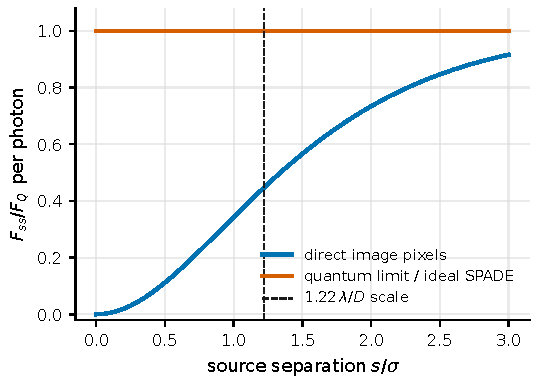
\includegraphics[width=0.82\linewidth]{figures/generated/chapter_08/ch08_rayleigh_information.pdf}
\caption{Separation information for two equally bright, incoherent Gaussian point sources. The blue curve is the direct-imaging Fisher information obtained by numerically integrating the image-plane probability density $p(x\mid s)$ (normalized to the quantum limit); at small separations it drops toward zero as $s^2$, which is the Rayleigh curse. The orange curve is the quantum limit of the next section, which remains finite even as $s\to0$. The vertical dashed line marks the commonly used Rayleigh angular scale.}
\label{fig:e12-rayleigh}
\end{figure}

\paragraph{Detection is not the same problem as estimation}
\label{sec:e12-detection}

Here we must draw a boundary that is easily overlooked. The whole Fisher-information apparatus above assumes by default that we have \emph{already accepted} the model "there are two equally bright stars up there," and simply do not know $s$. This is the estimation problem. Another class of problem is "is this really one star or two stars", this is called the \textbf{detection / model selection} problem. The two must not be conflated: in the detection problem the model dimension can change, and $s=0$ falls exactly on the \emph{boundary} of the parameter space, where the usual likelihood-ratio approximation (which assumes the parameter is at an interior point and the errors are near-Gaussian) need not hold; one must rely on simulation calibration or Bayesian evidence to decide. All the "sub-Rayleigh gains" discussed later in this chapter are, under the premise of an \emph{already accepted two-source model}, about reading the separation information already present in the light more cleanly, not about magically conjuring up a source out of nothing.

\paragraph{Multiple parameters: centroid, brightness ratio, and PSF width all compete for information}
\label{sec:e12-matrix}

In a real observation, the separation $s$ is never the only unknown. The centroid position $x_0$, the brightness ratio $r$ of the two stars, the PSF width $\sigma$, the background $b$\dots\ all must be estimated simultaneously. Then the scalar lower bound is upgraded to a \textbf{matrix} version. Arranging all parameters into a vector $\bm\theta=(s,x_0,r,\sigma,b,\dots)$, the Fisher information becomes a matrix:

\begin{equation}
  \mathrm{Cov}(\hat{\bm\theta})\ \succeq\ F^{-1},
  \qquad
  F_{\alpha\beta}=N_\gamma\int
  \frac{1}{p(x\mid\bm\theta)}
  \frac{\partial p}{\partial\theta_\alpha}
  \frac{\partial p}{\partial\theta_\beta}\,\mathrm{d}x.
  \label{eq:e12-fisher-matrix}
\end{equation}
\begin{formulaexplain}
$F_{\alpha\beta}$: the $(\alpha,\beta)$ element of the Fisher matrix, comparing the influence of parameters $\theta_\alpha$ and $\theta_\beta$ on the same data distribution. $\mathrm{Cov}(\hat{\bm\theta})\succeq F^{-1}$: the covariance matrix is no smaller than the inverse of the Fisher matrix (a matrix inequality). It is the diagonal elements of the inverse matrix that give the actual variances of the parameters.
\end{formulaexplain}

The crux is in \emph{taking the inverse}. The off-diagonal elements of $F$ record the \textbf{degeneracies} between parameters: if two parameters "look alike" in their effect on the data, their information becomes entangled, and after inversion the error is amplified. Concretely for sub-Rayleigh imaging: an unknown centroid mixes with the separation (shifting the whole image a little looks much like offsetting the two stars a little); an unknown brightness ratio redistributes information between the odd and even modes; an unknown PSF width is the most insidious: it and the binary separation both manifest as "the diffraction spot getting fatter" (recall the $s^2 h''$ term!), so the two are nearly collinear, and if $\sigma$ has not been independently calibrated tight, the binary signal will be absorbed as PSF broadening. So in reality, when reporting an error one cannot just throw out a single $1/\sqrt{F_{ss}}$; one must give the full covariance, plus the PSF calibration error, background error, and model error.


\section{Quantum Fisher information: putting the "measurement scheme" itself into the optimization}
\label{sec:e12-qfi}

At this point a sharp question surfaces: when the information of direct imaging drops toward zero, is it that the \emph{light itself} does not carry enough information, or that \emph{our measurement scheme} is too clumsy? The classical Fisher information~\eqref{eq:e12-fisher-def} is "fix the measurement scheme first (count photons pixel by pixel), then ask how much information is in the data." It takes the measurement as given. But quantum mechanics allows far more than "pixel by pixel", any orthogonal projection, any interference and mode decomposition counts.

We therefore introduce the \textbf{quantum Fisher information} (QFI): taking the optimum over \emph{all} measurements allowed by quantum mechanics, how much parameter information can in principle be read out at most from the same beam of light. It is the supremum of all classical Fisher informations, $F_{ss}\le F_{ss}^{Q}$. The QFI depends only on how the quantum state of the light field varies with the parameter, and not on which detector you choose.

To write down the state of this light, we borrow the weak-thermal-light conclusion of Chapter~\ref{chap:e06}. Celestial thermal light has a mean photon number $\epsilon\ll1$ per coherence-time mode, so the density matrix is approximately "vacuum plus a little single photon": $\rho\approx(1-\epsilon)|0\rangle\langle0|+\epsilon\,\rho_1$. That big chunk of vacuum does not click and carries no angular information: if no photon lands, you have no way to know how far apart the two stars are. What truly carries the separation information is the small fraction of detected \emph{single-photon spatial modes}. The single-photon part of two equally bright, incoherent point sources is an equal-weight mixture of two modes:

\begin{equation}
  \rho_{1}(s)=\tfrac12\,\big|\psi_{+s/2}\big\rangle\big\langle\psi_{+s/2}\big|
             +\tfrac12\,\big|\psi_{-s/2}\big\rangle\big\langle\psi_{-s/2}\big|,
  \label{eq:e12-one-photon}
\end{equation}
\begin{formulaexplain}
$\rho_1(s)$: the spatial-mode density matrix upon detecting one photon. $|\psi_{\pm s/2}\rangle$: the amplitude modes that the light of each star forms in the image plane after passing through the telescope (whose modulus squared is just the shifted PSF). Incoherent and equally bright $=$ an equal-weight probabilistic mixture of two single-photon states.
\end{formulaexplain}

Here $|\psi_{\pm s/2}\rangle$ is the amplitude PSF; for the Gaussian case $\psi(x)\propto\exp[-x^2/(4\sigma^2)]$ (its modulus squared $|\psi|^2\propto\exp[-x^2/(2\sigma^2)]=h$, with variance exactly $\sigma^2$).

Before formally throwing out the result, let us first let the reader nail down that key number for themselves. The magnitude of the QFI is ultimately determined by \emph{how easily the amplitude mode is distinguished under a shift}, and this is set by its "momentum variance" $\Delta k^2=\int(\psi')^2\,\mathrm{d}x$, a step that can be done by hand for a Gaussian. Differentiating the normalized $\psi(x)=(2\pi\sigma^2)^{-1/4}\exp[-x^2/(4\sigma^2)]$, we get $\psi'(x)=-\dfrac{x}{2\sigma^2}\psi(x)$, so
\[
  \Delta k^2=\int\big[\psi'(x)\big]^2\,\mathrm{d}x
  =\frac{1}{4\sigma^4}\int x^2\,|\psi(x)|^2\,\mathrm{d}x
  =\frac{1}{4\sigma^4}\cdot\sigma^2
  =\frac{1}{4\sigma^2},
\]
using $\int|\psi|^2\,\mathrm{d}x=1$ and $\int x^2|\psi|^2\,\mathrm{d}x=\sigma^2$ (the same Gaussian second moment). This $1/(4\sigma^2)$ is the origin of the surprisingly beautiful number in the single-photon QFI below. Under the ideal condition that the centroid, brightness, and PSF width are all known, computing the QFI rigorously for the rank-2 mixed state of Eq.~\eqref{eq:e12-one-photon}, the result is exactly $\Delta k^2$ per photon:

\begin{equation}
  F_{ss}^{Q}=N_\gamma\,\frac{1}{4\sigma^{2}}.
  \label{eq:e12-qfi}
\end{equation}
\begin{formulaexplain}
$F_{ss}^{Q}$: the \emph{upper limit} on separation information attainable by all allowed measurements. $\sigma$: the image-plane width corresponding to the amplitude mode. The crucial point is that it \emph{contains no $s$}: it does not vanish as $s\to0$, showing that the separation information sits safely in the light all along, and it is direct imaging that misses it.
\end{formulaexplain}

We need to \emph{honestly} tell the reader one thing: here we have only computed the "calibration scale" $\Delta k^2$, while treating the full proof of the rank-2 mixed-state QFI as a \textbf{known result to be cited}. It was founded by Helstrom's quantum estimation theory and given an explicit value for two-source sub-Rayleigh imaging by Tsang and collaborators, which we adopt directly here \citep{1969JSP.....1..231H,2016PhRvX...6c1033T}. The mixed-state QFI must be solved via the symmetric logarithmic derivative (SLD), and the rigorous derivation exceeds the undergraduate scope, so we do not expand it here; but the reader need not treat Eq.~\eqref{eq:e12-qfi} as "falling from the sky"; \S\ref{sec:e12-spade} will \emph{explicitly} construct the SPADE ruler and, step by step, compute the classical Fisher information up to the same $N_\gamma/(4\sigma^2)$. This confirms at least from below that $F_{ss}^{Q}\ge N_\gamma/(4\sigma^2)$ is attainable: since there exists a real measurement that reaches this value, the upper limit cannot possibly be lower.

Placing Eq.~\eqref{eq:e12-qfi} and the direct-imaging Eq.~\eqref{eq:e12-direct-fisher} side by side, the contrast is glaring:
\[
  \frac{F_{ss}^{\rm direct}}{F_{ss}^{Q}}
  =\frac{N_\gamma s^2/(8\sigma^4)}{N_\gamma/(4\sigma^2)}
  =\frac{s^2}{2\sigma^2}\ \xrightarrow{\,s\to0\,}\ 0.
\]
That is, in the sub-Rayleigh regime, the fraction of information that direct imaging uses tends to zero as $s^2$: the vast majority of information is thrown away for nothing (in Figure~\ref{fig:e12-rayleigh}, the blue curve dropping while the orange curve does not is exactly this). This is not the telescope circumventing diffraction, but the verdict of "putting the measurement scheme itself into the optimization": the information is in the light; it is a matter of whether you know how to read it \citep{1969JSP.....1..231H,2016PhRvX...6c1033T,2016OExpr..24.3684N}. The next section constructs that "reading" ruler.


\section{SPADE: translating a small separation into mode counts}
\label{sec:e12-spade}

The QFI only says "there exists an optimal measurement," not which one it is. For a Gaussian PSF and equally bright two sources, that optimal (or near-optimal) measurement has a concrete name: \textbf{spatial-mode demultiplexing} (SPADE). Its idea can be stated in one sentence: \emph{do not rush to ask which pixel the photon lands in; first ask which orthogonal spatial mode it belongs to, and then count photons in each mode separately}.

For a Gaussian PSF, the most natural set of orthogonal modes is the \textbf{Hermite--Gaussian modes}, denoted $u_0,u_1,u_2,\dots$. They are in fact old friends: the harmonic-oscillator eigenfunctions of Chapter~\ref{chap:e04}, a Gaussian times a Hermite polynomial, with $u_0$ a pure Gaussian, $u_1$ having one node, and $u_n$ having $n$ nodes. The fundamental mode $u_0$ can be taken to be exactly the amplitude PSF itself, $\psi(x)$.

\paragraph{Why the mode probabilities follow a Poisson distribution}
\label{sec:e12-poisson}

Now compute the probability that the light of one star (located at $+s/2$) lands in each mode. Its amplitude mode $\psi_{+s/2}(x)=\psi(x-s/2)$ is the fundamental mode \emph{shifted transversely} by $d=s/2$. Here we can borrow a beautiful correspondence from Chapter~\ref{chap:e04}: in the language of the harmonic oscillator, shifting the ground-state wavefunction in position by an amount $d$ yields exactly a \textbf{coherent state} $|\alpha\rangle$, and the occupation probability of a coherent state over number states (here just the mode index $n$) is a Poisson distribution $|\langle n|\alpha\rangle|^2=e^{-|\alpha|^2}|\alpha|^{2n}/n!$. The conversion between the displacement $d$ and $\alpha$ is $\alpha=d/(2x_{\rm zpf})$, and for our mode the zero-point fluctuation scale is $x_{\rm zpf}=\sigma$. So

\[
  |\alpha|^{2}=\frac{d^{2}}{4\sigma^{2}}
  =\frac{(s/2)^{2}}{4\sigma^{2}}
  =\frac{s^{2}}{16\sigma^{2}}\ \equiv\ Q.
\]

The other star at $-s/2$ has displacement $-d$, corresponding to $\alpha\to-\alpha$; but the Poisson probability depends only on $|\alpha|^2$, so positive and negative displacements give \emph{identical} mode probabilities. Hence for the equal-weight mixture of the two stars, the single-photon click probability in the $n$-th mode is

\begin{equation}
  p_{n}=e^{-Q}\,\frac{Q^{n}}{n!},
  \qquad
  Q=\frac{s^{2}}{16\sigma^{2}}.
  \label{eq:e12-spade-prob}
\end{equation}
\begin{formulaexplain}
$p_n$: the probability that a photon lands in the $n$-th Hermite--Gaussian mode. $Q$: the dimensionless "signal strength" built from the separation and the width, which is just the mean photon number of that equivalent coherent state. SPADE turns the continuous separation into a count distribution over a discrete set of modes.
\end{formulaexplain}

This Poisson shape uses the standard coherent-state result (Chapter~\ref{chap:e06}); if you would rather not borrow the harmonic oscillator, you can also directly compute the overlap integrals of the two shifted Gaussians with each Hermite--Gaussian mode, obtaining exactly the same $p_n$. Expanding at small $s$: $p_0=e^{-Q}\approx1-Q$ (almost all photons still in the fundamental mode), while
\[
  p_1=e^{-Q}Q\approx Q=\frac{s^{2}}{16\sigma^{2}},
\]
a small trickle of light leaks into the first (odd) mode $u_1$. This leakage is precisely the separation signal itself.

\paragraph{The count in the first mode, and why it circumvents the curse}
\label{sec:e12-mode-fisher}

Multiplying the probability by the photon number, the expected count in the first mode is

\begin{equation}
  \langle n_1\rangle\simeq N_\gamma\,\frac{s^{2}}{16\sigma^{2}}.
  \label{eq:e12-n1}
\end{equation}
\begin{formulaexplain}
$\langle n_1\rangle$: how many photons are expected in the first mode, equal to the total photon number times the probability $p_1$ of leaking into that mode. Small as the probability is, as long as $N_\gamma$ is large enough it can accumulate into a measurable count.
\end{formulaexplain}

Plug in real numbers. Take $s=0.1\sigma$ (well within the Rayleigh scale); then
\[
  Q=\frac{(0.1)^2}{16}=\frac{0.01}{16}=6.25\times10^{-4},
  \qquad p_1\approx6.25\times10^{-4}.
\]
Six in ten thousand: this sounds negligible. But if this bright star yields $N_\gamma=10^{8}$ source photons (a bright star can accumulate these in seconds to minutes), then in the ideal case there are $\langle n_1\rangle\approx6.3\times10^{4}$ photons in the first mode, more than enough signal-to-noise. Conversely, if the flux is only $N_\gamma=10^{5}$, the expected count is only about 63, and now dark counts, crosstalk, and background rise up to become the main limitations.

Now compute the Fisher information of the mode measurement and see how it circumvents the curse. The mode counts follow a Poisson/multinomial distribution, and their Fisher information is the weighted sum of the sensitivities of the mode probabilities to $s$:

\begin{equation}
  F_{ss}^{\rm mode}
  =N_\gamma\sum_{n}\frac{1}{p_n}
  \left(\frac{\partial p_n}{\partial s}\right)^{2}.
  \label{eq:e12-mode-fisher}
\end{equation}
\begin{formulaexplain}
$F_{ss}^{\rm mode}$: the separation Fisher information carried by the mode counts, the sum running over all spatial modes. Each term is the square of "the rate of change of the probability with $s$," divided by that mode's counting noise $p_n$.
\end{formulaexplain}

At small $s$ only the $n=1$ term matters. Using $p_1\approx s^2/(16\sigma^2)$ and its derivative $\partial p_1/\partial s\approx 2s/(16\sigma^2)=s/(8\sigma^2)$, substitute into that term:
\[
  \frac{1}{p_1}\left(\frac{\partial p_1}{\partial s}\right)^{2}
  =\frac{s^{2}/(64\sigma^{4})}{s^{2}/(16\sigma^{2})}
  =\frac{16\sigma^{2}}{64\sigma^{4}}
  =\frac{1}{4\sigma^{2}}.
\]
So

\begin{equation}
  F_{ss}^{\rm mode}\ \xrightarrow{\,s\to0\,}\ N_\gamma\,\frac{1}{4\sigma^{2}}
  \;=\;F_{ss}^{Q}.
  \label{eq:e12-mode-saturates}
\end{equation}
\begin{formulaexplain}
In the small-separation limit, the first mode alone pushes the Fisher information up to the quantum upper limit~\eqref{eq:e12-qfi}. SPADE therefore \emph{saturates} the quantum Fisher information, completely circumventing the Rayleigh curse.
\end{formulaexplain}

See clearly the mechanism of this "circumvention": $p_1$ itself shrinks as $s^2$ (weak signal), and $\partial p_1/\partial s$ shrinks as $s$ (weak slope too), but in the Fisher information it is "slope squared divided by probability," and $s^2/s^2$ \emph{cancels} exactly, leaving a finite value independent of $s$. Where does direct imaging fail? It projects photons onto position eigenstates, where the separation leaves only an $s^2$ broadening of shape (\S\ref{sec:e12-curse}), and the powers of $s$ in numerator and denominator do not match up, so it drops toward zero. SPADE switches to a different set of eigenstates (modes rather than positions), which happens to make the powers match \citep{2016PhRvX...6c1033T,2017NJPh...19b3054T}. Figure~\ref{fig:e12-spade-prob} plots the growth of the mode probabilities with $s/\sigma$, and Figure~\ref{fig:e12-direct-vs-modes} sets side by side the fact that "the image planes almost overlap while the mode counts have already separated."

\begin{figure}[tbp]
\centering
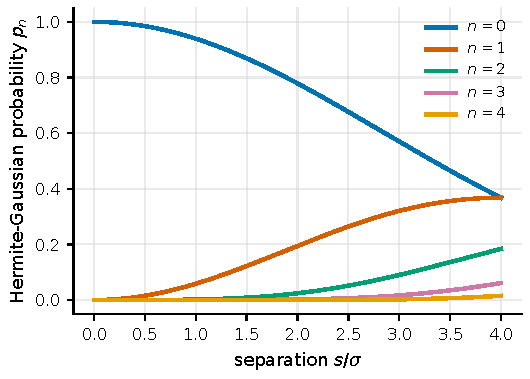
\includegraphics[width=0.82\linewidth]{figures/generated/chapter_08/ch08_spade_probabilities.pdf}
\caption{Mode probabilities for the ideal Hermite--Gaussian mode ordering. The horizontal axis is the separation $s/\sigma$, the vertical axis the single-photon probability of each mode. At small separations $p_0$ remains close to 1, while $p_1$ and the higher modes rise as powers of $Q=s^2/(16\sigma^2)$; the separation information is carried precisely by the counts of these low-probability modes.}
\label{fig:e12-spade-prob}
\end{figure}

\begin{figure}[tbp]
\centering
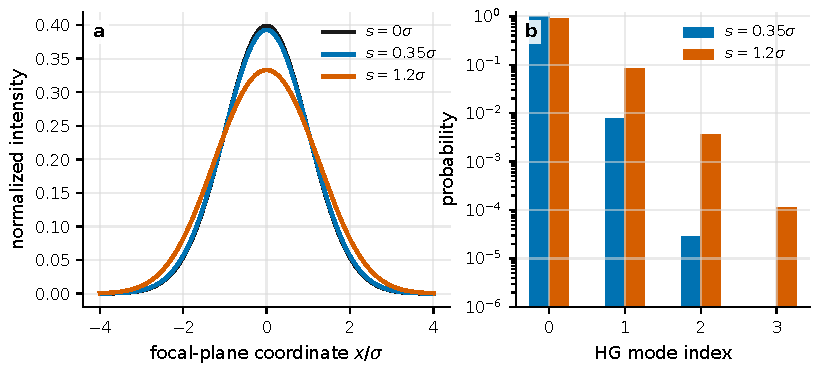
\includegraphics[width=0.92\linewidth]{figures/generated/chapter_08/ch08_direct_image_vs_modes.pdf}
\caption{The two faces of the same two-source model in the direct image and in the mode output. Left: the normalized image-plane intensity for $s=0$, $0.35\sigma$, $1.2\sigma$; in the sub-Rayleigh regime the curves differ only by an extremely weak broadening. Right: the probabilities of the first four Hermite--Gaussian modes at $s=0.35\sigma$ and $1.2\sigma$; small as the low-order non-fundamental-mode probabilities are, they turn the separation into perfectly clear mode counts.}
\label{fig:e12-direct-vs-modes}
\end{figure}


\section{Real-world limitations: the quantum bound is not automatically attainable}
\label{sec:e12-reality}

The beautiful Eq.~\eqref{eq:e12-mode-saturates} has one big premise: the mode basis is aligned exactly with the true centroid, and the mode sorter has no crosstalk and no background leakage. In reality all of these must be discounted, and the quantum bound is held up by a layer of \textbf{systematic floor}.

The most deadly is the \textbf{centroid / pointing error}. SPADE's first mode $u_1$ holds the signal through "the transverse asymmetry of the whole image relative to the mode centre." But if the whole image is shifted by $\delta x$ overall due to pointing jitter or tracking error, then this shift \emph{itself} pours light into $u_1$, and by exactly the same mechanism as the true signal. Using the same coherent-state conversion as the previous section, the fraction of an overall shift $\delta x$ leaking into the first mode is
\[
  p_1^{\rm leak}\approx\frac{\delta x^{2}}{4\sigma^{2}},
\]
while the true binary signal is $p_1^{\rm sig}\approx s^2/(16\sigma^2)$. The condition for the two to be equal is
\[
  \frac{\delta x^{2}}{4\sigma^{2}}=\frac{s^{2}}{16\sigma^{2}}
  \ \Longrightarrow\ \delta x=\frac{s}{2}.
\]
In other words, as soon as the centroid calibration error reaches half the separation, the spurious signal is of the same order as the true signal, and then the first-mode count you measure simply cannot distinguish "two stars" from "the telescope being misaligned." To measure a separation of $s=0.1\sigma$, one must stabilize and calibrate the centroid to far better than $0.05\sigma$, a very hard requirement on pointing, tracking, and calibration.

Beyond this there is a string of real-world killers: the \textbf{crosstalk} matrix of the mode sorter is unstable and leaks a little of the strong $u_0$ light into $u_1$, drowning the few-parts-in-ten-thousand signal; \textbf{background light}, if it does not have the same spatial-mode distribution as the source, lays a floor of noise across all modes; an insufficient Strehl ratio, aberrations drifting with time, dispersion, and polarization crosstalk all contaminate the mode response matrix. The common feature of these effects is that they \emph{do not decrease with $N_\gamma$}. The statistical error falls all the way down as $1/\sqrt{N_\gamma}$, but once it hits the systematic floor, adding more photons does not help (the green curve in Figure~\ref{fig:e12-crb} that flattens once calibration error is added is exactly this). So "reaching the quantum bound" is never automatic; experimentally, the more common approach is a simpler, more robust phase-sensitive measurement (a phase plate, SLIVER, SPLICE, and the like), which mitigates the quadratic loss of direct imaging, but whose actual gain is still dictated by visibility, crosstalk, and alignment error \citep{2017PhRvL.118g0801T,2019NJPh...21i3010B,2018Optic...5.1177P}.

\begin{figure}[tbp]
\centering
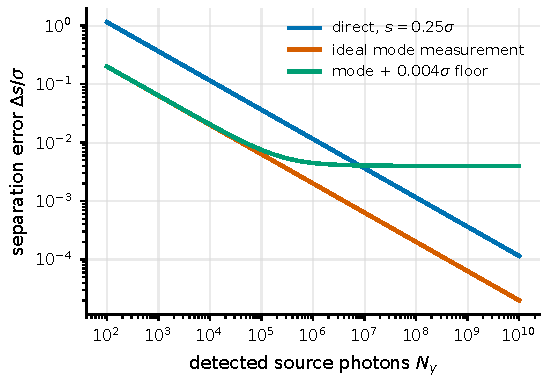
\includegraphics[width=0.82\linewidth]{figures/generated/chapter_08/ch08_cramer_rao_bound.pdf}
\caption{Cramér--Rao separation error for a sub-Rayleigh two-source system. The horizontal axis is the number of detected source photons $N_\gamma$, the vertical axis $\Delta s/\sigma$. The ideal mode measurement falls all the way down as $N_\gamma^{-1/2}$; direct imaging, with much smaller Fisher information, needs many more photons to catch up. The green curve, after adding a small piece of mode-matching systematic error, develops a plateau: continuing to add photons cannot remove the calibration error.}
\label{fig:e12-crb}
\end{figure}

There is a subtler premise still: the \textbf{partial coherence} of the source. Throughout the above we assumed the two stars are mutually incoherent (an equal-weight probabilistic mixture). Larson and Saleh pointed out that as the source becomes partially coherent, the Rayleigh curse may \emph{reappear}; Tsang and Nair subsequently clarified that as long as it is not the degenerate case of fully positive correlation, and one performs the correct Fisher computation for weak thermal light, SPADE still avoids the total vanishing of small-separation information \citep{2018Optic...5.1382L,2019Optic...6..400T}. In astronomy one must especially distinguish two things: whether two emitting regions on the source surface \emph{themselves} radiate independently, and the spatial coherence built up after the light propagates to the telescope by the van Cittert--Zernike theorem (Chapter~\ref{chap:e10}), are two different matters. The latter is precisely the quantity that interferometry measures, and cannot be simply equated with the coherence of the source's own emission.


\section{The long-baseline version: intensity interferometry does the same thing in the Fourier plane}
\label{sec:e12-sii}

The previous sections dealt with spatial-mode measurement at a single aperture, or after coherent beam combination. But this whole idea of "treating resolution as an estimation problem" can be carried over entirely to kilometre-scale long-baseline arrays, only this time the stage shifts from the image plane to the \textbf{Fourier plane}. Chapters~\ref{chap:e10} and~\ref{chap:e11} explained: the baseline between different pairs of telescopes samples different spatial frequencies of the sky brightness distribution; the constraint on the data comes from \emph{how the visibility varies with baseline}. Here "sub-Rayleigh" is no longer about reading two peaks out of one diffraction spot, but about measuring the Fourier modulus of the source brightness distribution on a long baseline.

Intensity interferometry does not measure the first-order field phase but the correlation of the intensity \emph{fluctuations} of two telescopes. Under ideal thermal light, the second-order correlation at zero delay (the Siegert/HBT relation of Chapter~\ref{chap:e10}) gives

\begin{equation}
  g_{ij}^{(2)}(0)-1=\big|\gamma_{ij}\big|^{2},
  \label{eq:e12-hbt}
\end{equation}
\begin{formulaexplain}
$g_{ij}^{(2)}(0)$: the zero-delay second-order correlation of telescopes $i,j$; subtracting 1 gives the excess relative to a "completely uncorrelated" baseline. $\gamma_{ij}$: the normalized complex degree of coherence, equal to the first-order visibility $V$. The degree of synchrony of the intensity fluctuations directly gives the squared visibility amplitude.
\end{formulaexplain}

The observable is therefore a series of squared visibilities across baselines/spectral channels/time intervals:

\begin{equation}
  d_{k}=\big|V(u_k,v_k;\bm\theta)\big|^{2}+\eta_{k},
  \label{eq:e12-sii-data}
\end{equation}
\begin{formulaexplain}
$d_k$: the squared visibility measured on the $k$-th baseline/time/spectral channel. $V$: the model visibility determined by the source parameters $\bm\theta$. $\eta_k$: the noise. The angular structure is written into how $|V|^2$ varies with baseline.
\end{formulaexplain}

Apply the same Cramér--Rao logic. For a parameter $\theta_\alpha$, the Fisher matrix of intensity interferometry is

\begin{equation}
  F_{\alpha\beta}^{\rm SII}
  =\sum_{k,l}
  \frac{\partial|V_k|^{2}}{\partial\theta_\alpha}\,
  C^{-1}_{kl}\,
  \frac{\partial|V_l|^{2}}{\partial\theta_\beta},
  \label{eq:e12-sii-fisher}
\end{equation}
\begin{formulaexplain}
$F_{\alpha\beta}^{\rm SII}$: the Fisher matrix of the intensity-interferometry data. $C^{-1}_{kl}$: the inverse of the measurement-error covariance of $|V|^2$, weighting the data points. The steeper the dependence of the squared visibility on a parameter, and the smaller its error, the more information.
\end{formulaexplain}

Here $C_{kl}$ is the covariance of the measurement error of $|V|^2$, which can be estimated using time-shifted background, empty baselines, overnight repeat observations, or injected simulations. If the errors of the data points are approximately independent, $C$ becomes diagonal, and Eq.~\eqref{eq:e12-sii-fisher} reduces to "the sum of each point's slope squared divided by variance", the same thing as the single-parameter Eq.~\eqref{eq:e12-fisher-def}, only with a sum replacing the integral. The crux is that \emph{slope} $\partial|V|^2/\partial\theta$: it tells you which baseline is most useful.

Plug in a concrete model: a uniform-disk star. Its visibility is a first-order Bessel function (this comes from the Fourier transform of the disk brightness distribution, derived in Chapter~\ref{chap:e10}):

\begin{equation}
  V(x)=\frac{2J_1(x)}{x},
  \qquad x=\frac{\pi B\theta_\star}{\lambda},
  \label{eq:e12-uniform-disk}
\end{equation}
\begin{formulaexplain}
$V(x)$: the visibility of a uniform disk. $J_1$: the first-order Bessel function. $B$: the projected baseline (metres). $\theta_\star$: the angular diameter of the star. The baseline scans the Fourier modulus of the disk through the dimensionless $x$.
\end{formulaexplain}

$V(x)$ equals 1 at $x=0$, decreases as $x$ grows to its first zero (the first nontrivial zero of $J_1$ is at $x\approx3.83$, the standard Bessel zero), and then turns over into a series of progressively weaker sidelobes. The most useful baseline for the angular diameter $\theta_\star$ falls where the slope $\partial|V|^2/\partial\theta_\star$ of $|V|^2$ is largest, usually along the section where the visibility drops rapidly. On short baselines $V\approx1$ and barely varies with $\theta_\star$ (no slope on the plateau, no information); on extremely long baselines the signal falls into the sidelobes and is easily overwhelmed by systematic errors. So "longer baseline is not always better"; rather, one should \emph{choose where the slope is large}. Figure~\ref{fig:e12-sii-fisher} plots this design principle very plainly.

\begin{figure}[tbp]
\centering
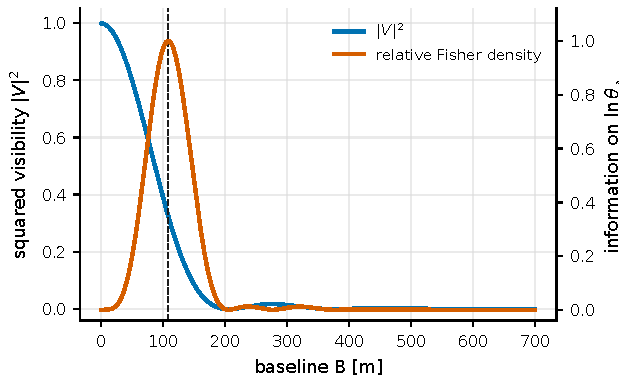
\includegraphics[width=0.82\linewidth]{figures/generated/chapter_08/ch08_visibility_fisher_design.pdf}
\caption{The relation between baseline choice and parameter information in intensity interferometry. The blue curve is the squared visibility of a uniform disk with $\lambda=450~\mathrm{nm}$ and $\theta_\star=0.55~\mathrm{mas}$; the orange curve is the Fisher weight computed from $\partial|V|^2/\partial\ln\theta_\star$ and normalized. The most useful baseline falls where the visibility drops rapidly; simply lengthening or shortening the baseline does not automatically add angular-diameter information.}
\label{fig:e12-sii-fisher}
\end{figure}

The price of intensity interferometry is \textbf{phase loss}: $|V|^2$ discards the phase of $V$, and is therefore insensitive to overall translation and brings mirror and central-symmetry degeneracies: the orientation of a binary, the position of a bright spot, or an asymmetric disk often must be mitigated by the $uv$ coverage from Earth's rotation, multiple wavelengths, prior models, or third-order correlations. What it buys in return is enormous: near-immunity to atmospheric phase disturbances. Because it only compares whether the \emph{intensity} fluctuations of the two paths are synchronous, the telescopes need only an electronic connection and to align their signals in time to a small fraction of the detector response, without maintaining optical coherence (Chapter~\ref{chap:e10} showed that nanosecond-level electronic timing corresponds to a path-length tolerance of tens of centimetres, and the atmospheric piston jitter of a few nanometres falls entirely within that tolerance). For exactly this reason, atmospheric Cherenkov telescope arrays (whose optical image quality is far inferior to that of professional interferometers but which enjoy large collecting area and long baselines) turn out to be ideal intensity-interferometry arrays \citep{1956Natur.177...27B,1974MNRAS.167..121H,2020NatAs...4.1164A,2024MNRAS.529.4387A}.

\paragraph{The division of labour between the two engineering routes}
\label{sec:e12-two-roads}

Placing the two kinds of "sub-Rayleigh estimation" side by side, their engineering bottlenecks are exactly opposite, and so their suitable targets differ:

\begin{itemize}
  \item \textbf{SPADE / spatial-mode measurement} (single aperture or coherent beam combination): requires a \emph{stable wavefront}. The target light must be coupled into fibre modes, an integrated-optics chip, or a free-space mode sorter, with adaptive optics squeezing the incident light into as few controllable modes as possible. Its enemies are the Strehl ratio, non-common-path aberrations, centroid jitter, and mode crosstalk. It suits few-parameter problems such as reading the angular separation of two nearby stars or the low-order shape moments of a star.
  \item \textbf{Intensity interferometry} (long-baseline arrays): simply \emph{accepts} that the atmosphere randomizes the phase, and trades large collecting area and long baselines for $|V|^2$ information. Its enemies are low photon rate, electronic bandwidth, background, time synchronization, and systematic covariance. It suits bright hot stars, rapid rotators, binaries, and angular-diameter measurements.
\end{itemize}

Whichever route one takes, a publishable sub-Rayleigh estimate must present four sets of accounts at once: the \emph{photon budget} (magnitude, spectral band, total efficiency, exposure $\to$ effective $N_\gamma$); the \emph{angular scale} ($\lambda/D$, PSF width $\sigma_\theta$, candidate separation $s$ or angular diameter $\theta_\star$); the \emph{measurement matrix} (pixel response, mode crosstalk, or the $|V|^2$ covariance); and the \emph{model boundaries and error decomposition} (how equally bright two sources, an unknown brightness ratio, a finite disk, partial coherence, or a background star rewrite the Fisher matrix). Finally, checking one criterion is enough to diagnose: is the statistical error still falling as $N_\gamma^{-1/2}$? If it is no longer falling, chances are that alignment, PSF, background, correlator, or model errors have hit a plateau. Putting these boundaries into the final inference commonly uses Bayesian sampling and evidence comparison: direct-imaging, mode-count, and intensity-interferometry data can share the same parameter vector, with joint likelihoods multiplied; priors such as a known orbit, colour, spectral type, and distance directly reshape the identifiable parameter space \citep{2009MNRAS.398.1601F,2013PASP..125..306F}.


\section{Chapter Summary}
\label{sec:e12-summary}

\begin{itemize}
  \item \textbf{Resolution is an estimation problem, not an imaging criterion.} The Rayleigh criterion $\theta_{\rm R}=1.22\lambda/D$ only asks "can the image plane be split into two peaks"; the real question to ask is "given $N_\gamma$ photons, how precisely can the separation $s$ be estimated," and the answer is given by the Fisher information and the Cramér--Rao bound $\mathrm{Var}(\hat s)\ge1/F_{ss}$.
  \item \textbf{At small separations, the first effect is fattening, not splitting.} Taylor-expanding the two shifted PSFs, the first-order terms cancel and $p(x\mid s)=h+\tfrac{s^2}{8}h''+\mathcal O(s^4)$. The separation appears at lowest order as a second-order broadening through $h''$, and the direct-imaging Fisher information $F_{ss}^{\rm direct}\simeq N_\gamma s^2/(8\sigma^4)\to0$: this is the Rayleigh curse.
  \item \textbf{The information never leaves the light.} The quantum Fisher information replaces "pixel by pixel" with "all allowed measurements," giving for the weak-thermal single-photon state $F_{ss}^{Q}=N_\gamma/(4\sigma^2)$, which does not vanish as $s\to0$. The curse is a disease of the measurement scheme, not of the light.
  \item \textbf{SPADE saturates the quantum limit.} Projecting onto Hermite--Gaussian modes and then counting, the mode probabilities follow a Poisson distribution $p_n=e^{-Q}Q^n/n!$ with $Q=s^2/(16\sigma^2)$. In the first mode $p_1\propto s^2$ and $\partial p_1/\partial s\propto s$, and their ratio in the Fisher information leaves the finite limit $N_\gamma/(4\sigma^2)$, circumventing the curse.
  \item \textbf{The bound is not automatically attainable.} The amount of a centroid error $\delta x$ leaking into the first mode is $\delta x^2/(4\sigma^2)$, which becomes of the same order as the signal $s^2/(16\sigma^2)$ when $\delta x\sim s/2$; crosstalk, background modes, and partial coherence all create a systematic floor that does not decrease with $N_\gamma$.
  \item \textbf{The long baseline is the Fourier version of the same thing.} Intensity interferometry estimates parameters in the Fourier plane, $F^{\rm SII}_{\alpha\beta}=\sum\partial|V|^2/\partial\theta\,C^{-1}\,\partial|V|^2/\partial\theta$, and the most useful baseline is where the slope of $|V|^2$ is large. It discards the phase and is immune to the atmosphere, complementing SPADE's "stable-wavefront" route.
\end{itemize}

\medskip
\noindent\textbf{Questions to Ponder.}
\begin{enumerate}
  \item If the \emph{brightness ratio} of the two stars is also set as an unknown parameter, how much separation information remains in the first (odd) mode and in the fundamental (even) mode respectively? Why does the degeneracy of an "unknown brightness ratio" weaken the contribution of the odd mode?
  \item The direct-imaging result $F_{ss}^{\rm direct}\propto s^2$ was derived under a \emph{Gaussian} PSF. If one switches to an Airy PSF with real sidelobes, does the second-order broadening step change? Is the Rayleigh curse a peculiarity of the Gaussian, or a more general phenomenon?
  \item Intensity interferometry discards the phase, while SPADE retains information on the relative phase of the modes. For the task of "measuring the \emph{orientation} of two nearby stars," which has the advantage? Translate it into the degeneracy in Eq.~\eqref{eq:e12-sii-fisher} to explain.
\end{enumerate}
